%moving car using graphics.h
\documentclass[12pt]{article}

\usepackage{amsmath}
\usepackage{graphicx}
\usepackage[a4paper]{geometry}

\geometry{
  textwidth=\dimexpr\paperwidth-29mm,
  textheight=\dimexpr\paperheight-32mm,
  noheadfoot,
  nomarginpar
}

\setlength{\topskip}{0mm}
\setlength{\parindent}{0mm}

\title{Animation of a Moving Car using graphics.h in C}
\date{}
\author{}

\begin{document}
	\maketitle
	\vspace{-2cm}

	\section{Objective}
	To create an animation of a moving car using graphics.h in C.
	\section{Theory}
	We have learned the basics of graphics.h in C. 
	Using the concept of redrawing a frame multiple times in a loop with a delay adjusted for the human eye, we can create the simple animations such as a moving car implemented as below.

    \section{Algorithm}
    \begin{enumerate}
        \item Initialize graphics using \texttt{initgraph()} function.
        \item Start a loop that runs 500 times (adjust the loop count for desired animation duration).
        \item Draw the road using \texttt{line()} function.
        \item Draw the car using various shapes like rectangles, lines, and circles to represent different parts of the car.
        \item Move the car horizontally by incrementing the x-coordinates of its components within the loop.
        \item Add a delay using \texttt{delay()} function to control the animation speed.
        \item Clear the screen using \texttt{cleardevice()} function to prepare for the next frame.
        \item End the loop.
    \end{enumerate}


	\section{Source Code}
\begin{verbatim}
#include "labs.h"
#include "definitions.h"

int main()
{	
    int gd = DETECT, gm;
    initgraph(&gd, &gm, "");
    setcolor(GREEN);

    while(1)
    {
        // lab5();
        car();
    }

    getch();
    closegraph();
    return 0;
}

void car()
{
    int car[][2] =
    {
        {0, 0},
        {0, 30},
        {-30, 30},
        {-30, 60},
        {-90, 60},
        {-90, 30},
        {-90, 30},
        {-120, 30},
        {-120, 0},
    };
    unsigned size = sizeof(car) / sizeof(car[0]);
    drawObject(size, car);
    int wheelCoords[] = { -30, 0, 10 };
    int wheelCoords2[] = { -90, 0, 10 };
    translateAxes(&wheelCoords[0], &wheelCoords[1]);
    translateAxes(&wheelCoords2[0], &wheelCoords2[1]);

    // draw road
    // translation stuff
    for(size_t i = 0; i < 200; i++)
    {
        cleardevice();
        translate(size, car, 1, 0);
        translateArr(1, wheelCoords, 1);
        translateArr(1, wheelCoords2, 1);
        circle(wheelCoords[0], wheelCoords[1], wheelCoords[2]);
        circle(wheelCoords2[0], wheelCoords2[1], wheelCoords2[2]);
        drawObject(size, car);
        line(0, HEIGHT / 2, WIDTH, HEIGHT / 2);
        line(0, HEIGHT / 2 + 30, WIDTH, HEIGHT / 2 + 30);
        delay(10);
    }
    delay(500);
}
\end{verbatim}

	\newpage
	\section{Output}

	\begin{figure}[!h]
		\hspace*{-1cm}
		\centering
		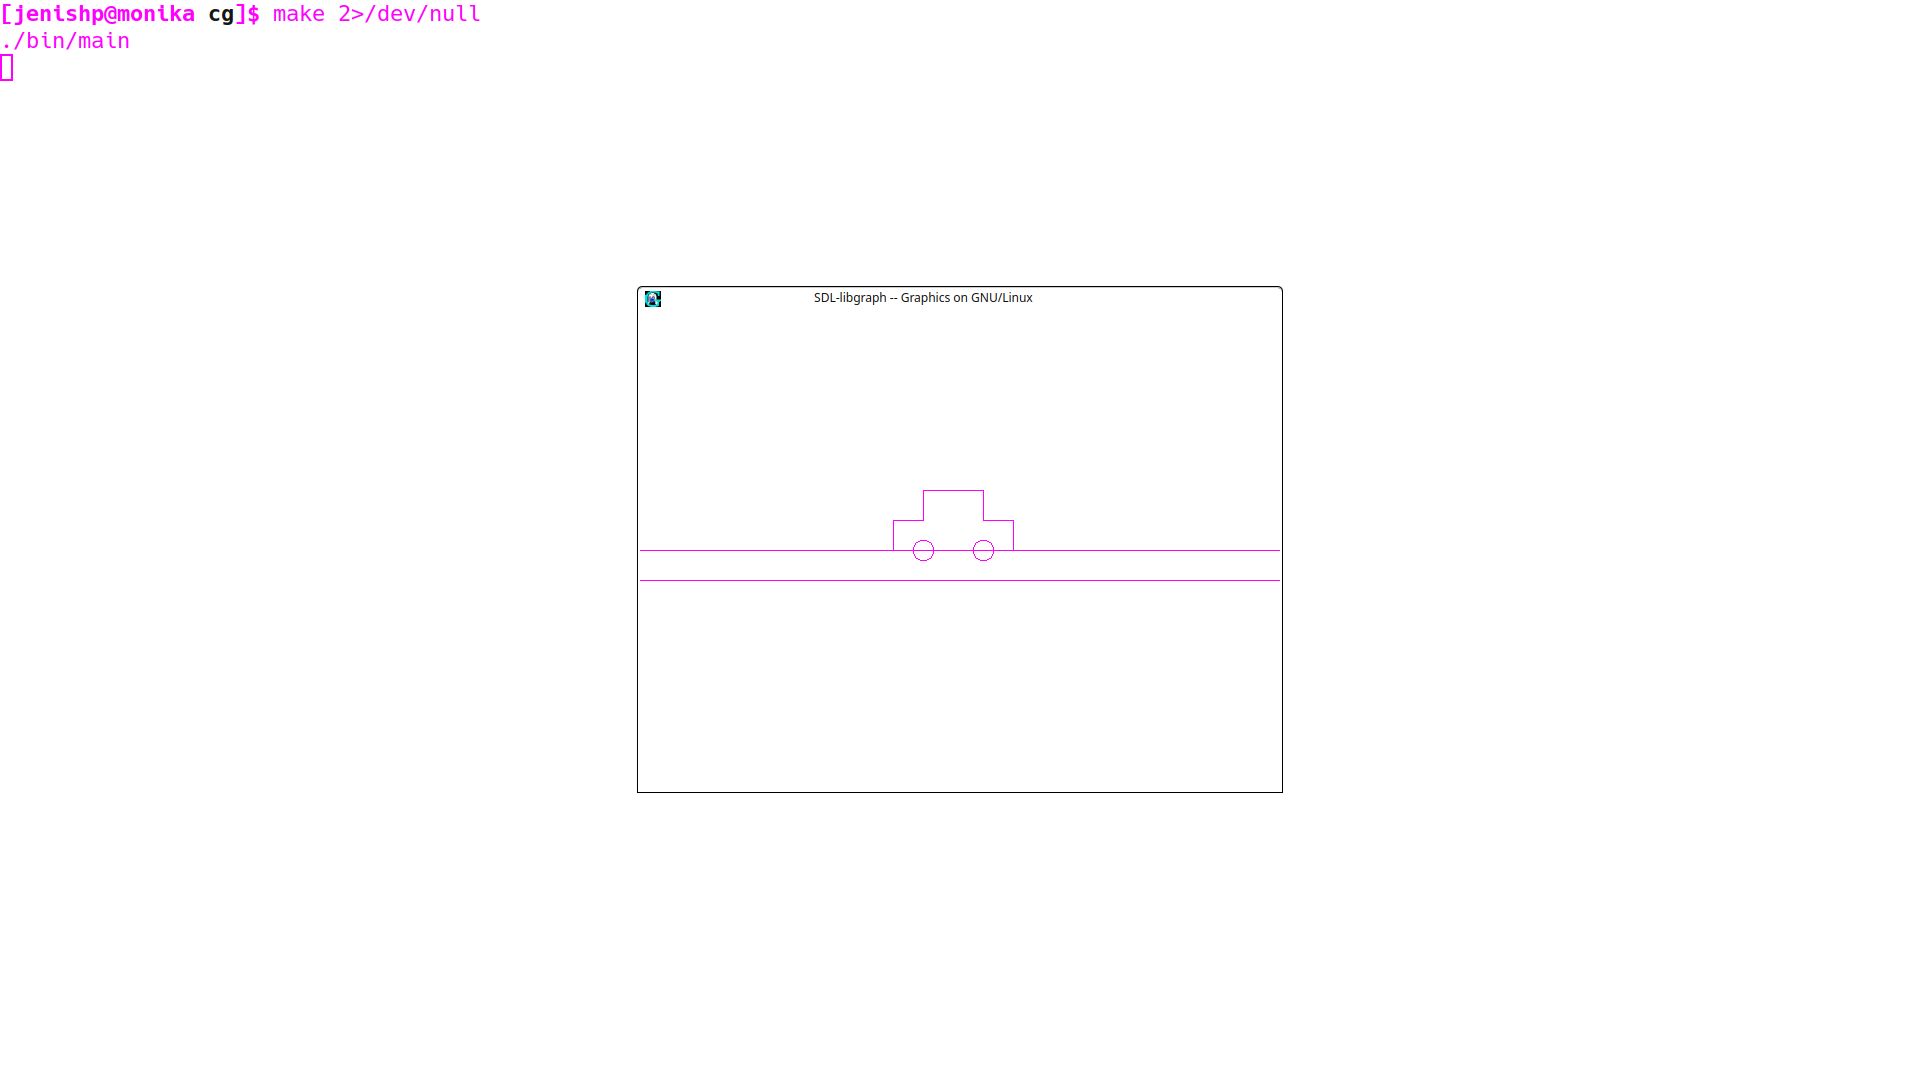
\includegraphics[width=1.01\linewidth]{output1.png}
		\caption{Initial State of the car}
		\label{fig:}
	\end{figure}

	\begin{figure}[!h]
		\hspace*{-1cm}
		\centering
		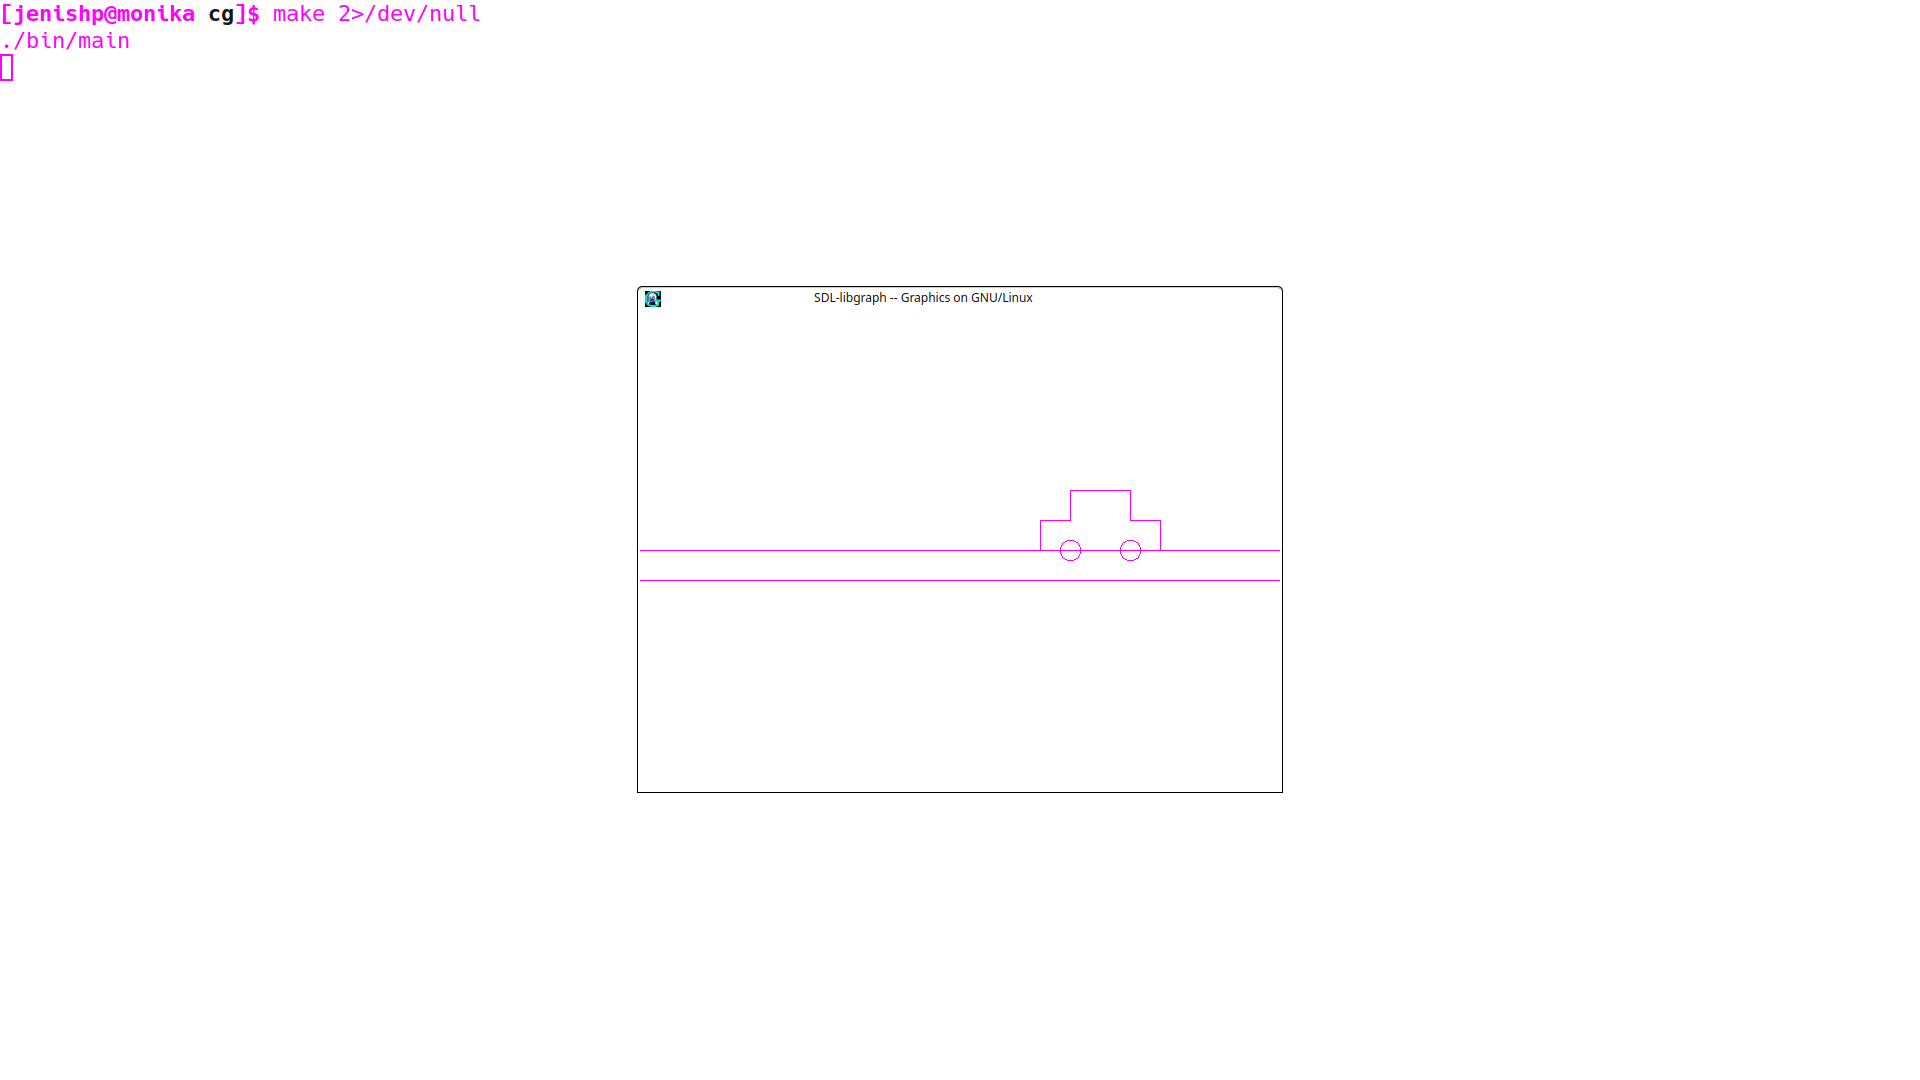
\includegraphics[width=1.01\linewidth]{output2.png}
		\caption{Final State of the car(After continuous translation)}
		\label{fig:}
	\end{figure}

	\section{Conclusion}
	We have successfully created an animation of a moving car using graphics.h in C.
	Using the functions and algorithms previously learned, we were able to create this simple animation.
	Using the same concept, we can create more complex animations and games.

\end{document}


